
\documentclass[a4paper]{article}

\usepackage{amsmath,amssymb,latexsym, marvosym}
\usepackage{tikz}
\usetikzlibrary{shapes,snakes}

\begin{document}


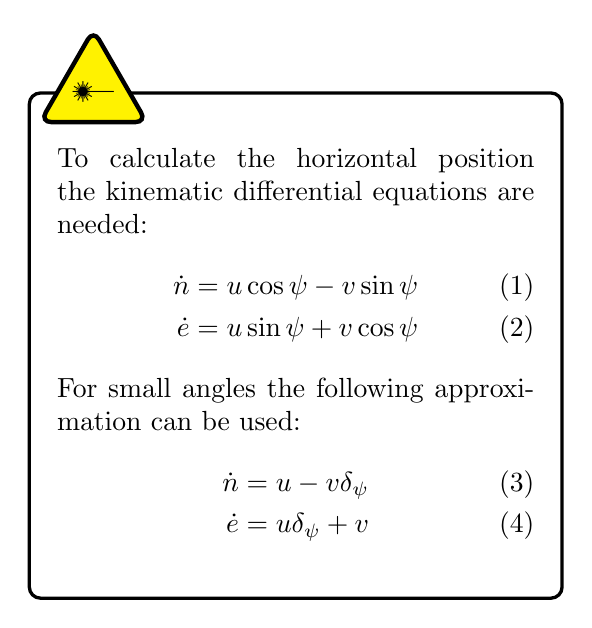
\begin{tikzpicture}

% Define box and box title style
\tikzstyle{mybox} = [draw=black, fill=white!20, very thick,
    rectangle, rounded corners, inner sep=10pt, inner ysep=20pt]
\tikzstyle{fancytitle} =[regular polygon, regular polygon sides=3,
           rounded corners, inner sep=0pt,
           draw=black, ultra thick, fill=yellow, text=black]

\node [mybox] (box){%
    \begin{minipage}{0.50\textwidth}
        To calculate the horizontal position the kinematic differential
        equations are needed:
        \begin{align}
            \dot{n} &= u\cos\psi -v\sin\psi \\
            \dot{e} &= u\sin\psi + v\cos\psi
        \end{align}
        For small angles the following approximation can be used:
        \begin{align}
            \dot{n} &= u -v\delta_\psi \\
            \dot{e} &= u\delta_\psi + v
        \end{align}
    \end{minipage}
};


\node[fancytitle, right = 10pt] at (box.north west) {\Laserbeam};
\end{tikzpicture}%

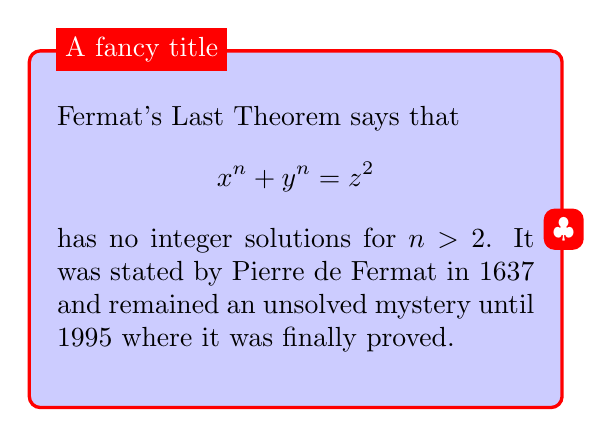
\begin{tikzpicture}%
\tikzstyle{mybox} = [draw=red, fill=blue!20, very thick,
    rectangle, rounded corners, inner sep=10pt, inner ysep=20pt]
\tikzstyle{fancytitle} =[fill=red, text=white]

\node [mybox] (box){%
    \begin{minipage}{0.50\textwidth}
     Fermat's Last Theorem says that
      $$
          x^n + y^n = z^2
      $$
     has no integer solutions for $n>2$. It was stated by
    Pierre de Fermat in 1637 and remained an unsolved mystery
    until 1995 where it was finally proved.
    \end{minipage}
};
\node[fancytitle, right=10pt] at (box.north west) {A fancy title};
\node[fancytitle, rounded corners] at (box.east) {$\clubsuit$};
\end{tikzpicture}%


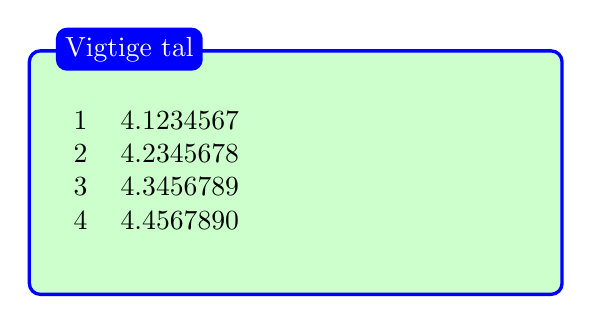
\begin{tikzpicture}%
\tikzstyle{mybox} = [draw=blue, fill=green!20, very thick,
    rectangle, rounded corners, inner sep=10pt, inner ysep=20pt]
\tikzstyle{fancytitle} =[fill=blue, rectangle, rounded corners, text=white]

\node [mybox] (box){%
    \begin{minipage}{0.50\textwidth}
      \begin{tabular}{ll}
         1 & 4.1234567 \\
         2 & 4.2345678 \\
         3 & 4.3456789 \\
         4 & 4.4567890 \\
      \end{tabular}
    \end{minipage}
};
\node[fancytitle, right=10pt] at (box.north west) {Vigtige tal};
\end{tikzpicture}%


\end{document}
